\documentclass[11pt]{article}

% ── Packages ────────────────────────────────────────────────────────────────
\usepackage[utf8]{inputenc}
\usepackage[T1]{fontenc}
\usepackage[margin=1in]{geometry}
\usepackage{amsmath,amssymb}
\usepackage{graphicx}
\graphicspath{{figures/}}
\usepackage{subcaption}
\captionsetup[figure]{labelfont=it}
\usepackage{float}
\usepackage{placeins}
\usepackage{booktabs}
\usepackage{tabularx}
\usepackage{siunitx}
\usepackage{xcolor}
\usepackage{listings}
\usepackage{microtype}
\usepackage{hyperref}
\hypersetup{
    colorlinks = true,
    linkcolor  = blue!50!black,
    citecolor  = black,
    urlcolor   = blue!50!black,
}
\usepackage{cleveref}
\usepackage{tikz}
\usetikzlibrary{arrows.meta,shapes.geometric,positioning,calc,decorations.pathreplacing}
\usepackage{pgfplots}
\pgfplotsset{compat=1.18}

% ── Code listing style ─────────────────────────────────────────────────────
\definecolor{codebg}{RGB}{247,247,250}
\definecolor{codekeyword}{RGB}{0,33,165}
\definecolor{codecomment}{RGB}{110,110,110}
\definecolor{codestring}{RGB}{160,30,30}

\lstdefinestyle{pythonstyle}{
    language=Python,
    backgroundcolor=\color{codebg},
    basicstyle=\ttfamily\scriptsize,
    keywordstyle=\color{codekeyword}\bfseries,
    commentstyle=\color{codecomment}\itshape,
    stringstyle=\color{codestring},
    numbers=left,
    numberstyle=\tiny\color{gray},
    numbersep=8pt,
    frame=single,
    rulecolor=\color{black!20},
    breaklines=true,
    breakatwhitespace=false,
    showstringspaces=false,
    tabsize=4,
    captionpos=b,
    columns=fullflexible,
    keepspaces=true,
}
\lstset{style=pythonstyle}

% ── Program output style (plain monospace, no line numbers) ─────────────────
\lstdefinestyle{outputstyle}{
    language={},
    basicstyle=\ttfamily\scriptsize,
    backgroundcolor=\color{codebg},
    frame=single,
    rulecolor=\color{black!20},
    numbers=none,
    columns=fixed,
    tabsize=8,
}
\newcommand{\programoutput}[2][]{\lstinputlisting[style=outputstyle,#1]{#2}}

% ── Colors used in the figures (match the handwritten diagrams) ────────────
\definecolor{hwpurple}{RGB}{90,45,145}
\definecolor{hwmagenta}{RGB}{230,0,200}
\definecolor{hwblue}{RGB}{20,70,190}
\definecolor{hwred}{RGB}{225,30,30}
\definecolor{hwgreen}{RGB}{0,130,70}

% ── Vector notation (underbar, matching handwritten convention) ────────────
\newcommand{\vect}[1]{\underline{#1}}
\newcommand{\ivect}[1]{{}^{I}\underline{#1}}   % inertial-frame vector, e.g. {}^I v

% ── Divider page (used for the appendix section-break) ─────────────────────
\newcommand{\dividerpage}[3]{%
    \clearpage
    \thispagestyle{empty}
    \begin{center}
        \vspace*{\fill}
        {\Huge\bfseries #1\par}
        \vspace{1cm}
        {\Large #2\par}
        \vspace{1.5cm}
        {\normalsize #3\par}
        \vspace*{\fill}
    \end{center}
    \clearpage
}

% ── Source code link ────────────────────────────────────────────────────────
\newcommand{\repolink}{\url{https://github.com/PabloCoralDev/Astrodynamics-Project-3}}

\title{EAS4510, Project \#3}
\author{Pablo Coral}
\date{\today}

\begin{document}

% ── Cover page ───────────────────────────────────────────────────────────
\pagenumbering{roman}
\begin{titlepage}
    \centering
    \vspace*{3cm}
    {\LARGE\bfseries Apoapsis Dwell Orbit Design for USSPACECOM\par}
    \vspace{0.5cm}
    {\Large EAS4510, Project \#3\par}
    \vspace{1.5cm}
    {\Large Pablo F. Coral\par}
    \vspace{0.5cm}
    {\large \today\par}
    \vspace{1cm}
    {\normalsize GitHub: \repolink\par}
    \vfill
    
\includegraphics[width=\textwidth]{honor_code.png}
    \vspace*{1cm}
\end{titlepage}
\clearpage
\pagenumbering{arabic}
\setcounter{page}{1}

\section{Task 1: Apoapsis Dwell Orbit in Inertial Space}
\label{sec:task1}

\begin{newpar}
USSPACECOM has specified an orbit with the following parameters:
\begin{equation}
T = \SI{24}{\hour}, \qquad e = 0.25, \qquad i = 63.4^\circ, \qquad \omega = \{90^\circ, 270^\circ\}, \qquad 0 \le \Omega \le 180^\circ,
\label{eq:t1-given}
\end{equation}
and with the spacecraft at periapsis at the epoch $t=t_0=0$. We can calculate the semi-major axis from the given period,
\begin{equation}
T = 2\pi\sqrt{\frac{a^3}{\mu}} \;\;\Longrightarrow\;\; a = \left(\frac{\mu T^2}{4\pi^2}\right)^{1/3},
\end{equation}
which we can use for $p = a(1-e^2)$, $r_p = p/(1+e)$, and $r_a = p/(1-e)$:
\end{newpar}

\begin{table}[H]
\centering
\caption{\newtxt{Fixed orbit design parameters, $\mu = \SI{398600}{\kilo\meter\cubed\per\second\squared}$.}}
\label{tab:t1-design}
\color{newtext}
\begin{tabular}{@{}lr@{\qquad}lr@{}}
\toprule
Quantity & Value & Quantity & Value \\
\midrule
$a$ [\si{\kilo\meter}] & $42241.0801$ & $p$ [\si{\kilo\meter}] & $39601.0126$ \\
$e$ [--] & $0.2500$ & $r_p$ [\si{\kilo\meter}] & $31680.8101$ \\
$i$ [\si{\degree}] & $63.4000$ & $r_a$ [\si{\kilo\meter}] & $52801.3501$ \\
$T$ [\si{\hour}] & $24.0000$ & $\Delta t$ [\si{\minute}] & $5$ \\
\bottomrule
\end{tabular}
\end{table}

\subsection*{Task 1-1: Kepler solver}

For an elliptic orbit ($0 \le e < 1$), the \newtxt{true anomaly} at an arbitrary time $t$ \newtxt{is} obtained from \newtxt{$\nu_0$}, $t_0$, $t$, and $\mu$ using the method of Section 3.5\newtxt{~\cite{course-notes}}:
\begin{enumerate}
    \item Solve for $E_0$ from $\nu_0$ using
    \begin{equation}
        E_0 = 2\tan^{-1}\!\left[\sqrt{1-e}\sin\!\left(\frac{\nu_0}{2}\right),\ \sqrt{1+e}\cos\!\left(\frac{\nu_0}{2}\right)\right].
        \label{eq:t1-E0}
    \end{equation}
    \item Solve the general form of Kepler's equation for $E(t)$ to obtain C:
    \begin{equation}
        E - e\sin E = \sqrt{\frac{\mu}{a^3}}(t-t_0) - 2\pi k + \big(E_0 - e\sin E_0\big) \equiv C,
        \label{eq:t1-kepler}
    \end{equation}
    using the fixed-point iteration
    \begin{equation}
        E^{(n+1)} = e\sin E^{(n)} + C,
        \label{eq:t1-fpi}
    \end{equation}
    with the suggested initial guess:
    \begin{equation}
        E^{(0)} = M_0 = E_0 - e\sin E_0,
    \end{equation}
    and run for the suggested number of iterations,
    \begin{equation}
        N = 10\left\lceil \frac{1}{1-e} \right\rceil.
    \end{equation}
    The integer $k$ is the number of periapsis crossings between $t_0$ and $t$, obtained from
    \begin{equation}
        k = \left\lfloor \frac{M_0 + \sqrt{\mu/a^3}\,(t-t_0)}{2\pi} \right\rfloor.
        \label{eq:t1-k}
    \end{equation}
    \item Recover the true anomaly at $t$ from the obtained $E$ (in step \newtxt{2}),
    \begin{equation}
        \nu = 2\tan^{-1}\!\left[\sqrt{1+e}\sin\!\left(\frac{E}{2}\right),\ \sqrt{1-e}\cos\!\left(\frac{E}{2}\right)\right].
        \label{eq:t1-nu}
    \end{equation}
\end{enumerate}
\newtxt{\texttt{step\_kepler(t\_prev, nu\_prev, t, a, e, mu)} in \texttt{kepler.py} implements these three steps.}

\subsection*{Task 1-2: True anomaly at a sequence of times}

\newtxt{The} time grid $\vect{t}$ is built and the true anomaly $\vect{N}$ is computed at each time. With $\Delta t = \SI{5}{\minute}$\newtxt{, $t_0 = 0$, $\nu_0 = 0$,} and $t_n = t_0 + \newtxt{T}$,
\begin{equation}
\vect{t} = \begin{bmatrix} t_0 & t_1 & \cdots & t_n \end{bmatrix}^T,\quad t_i = t_{i-1} + \Delta t
\;\;\Longrightarrow\;\;
n + 1 = 289 \text{ points}.
\end{equation}
\texttt{computeNu(t\_arr, \newtxt{nu\_0, a, e,} miu)} sets $\nu_0$ as the first element of $\vect{N}$, and then calls \texttt{\newtxt{step\_kepler}} once per step with $(t_{i-1},\nu_{i-1},t_i)$ to get $\nu_i$ ($i = 1,\dots,n$).

\subsection*{Task 1-3: Position and velocity}

With $\vect{N}$ from \newtxt{Task 1-2} and the orbital elements $(a,e,\Omega,i,\omega)$, the ECI position and inertial velocity are computed at every $\nu_j$. Each pair is first written in the perifocal frame $P$ (\cref{fig:t1-perifocal}), then rotated to the ECI frame $I$.

\begin{figure}[H]
\centering
% Redrawn from Project 2 Handwork p.4 (perifocal frame, r at true anomaly nu).
% Ellipse: a = 2.5, e = 0.6, b = 2, focus at the origin, nu = 60 deg -> r = 1.2308.
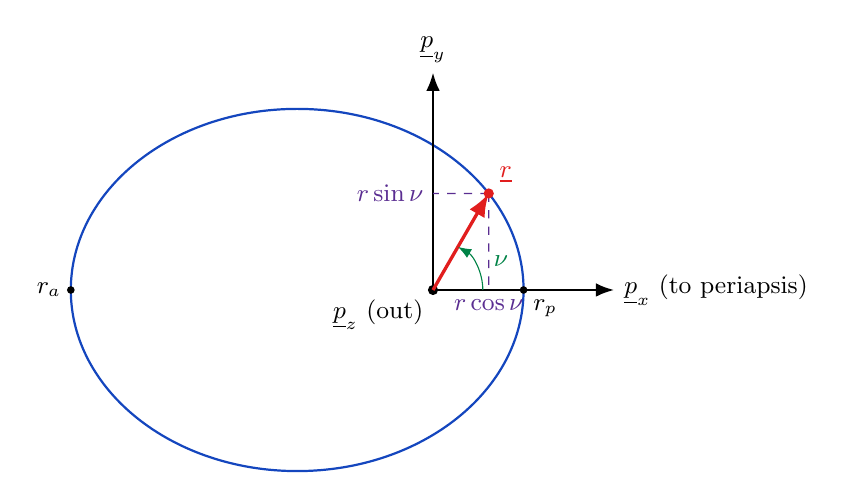
\begin{tikzpicture}[>=Latex, scale=1.15, font=\small]
    % orbit
    \draw[thick, hwblue] (-1.5,0) ellipse (2.5 and 2);
    \fill (0,0) circle (1.6pt);
    \node[below left] at (0,0) {$\vect{p}_z$ (out)};
    % perifocal axes
    \draw[->, thick] (0,0) -- (2.0,0) node[right] {$\vect{p}_x$ (to periapsis)};
    \draw[->, thick] (0,0) -- (0,2.4) node[above] {$\vect{p}_y$};
    % position vector and projections
    \coordinate (S) at (0.6154,1.0659);
    \draw[->, very thick, hwred] (0,0) -- (S) node[above right] {$\vect{r}$};
    \draw[dashed, hwpurple] (S) -- (0.6154,0) node[below] {$r\cos\nu$};
    \draw[dashed, hwpurple] (S) -- (0,1.0659) node[left] {$r\sin\nu$};
    \fill[hwred] (S) circle (1.6pt);
    % true anomaly
    \draw[->, hwgreen] (0.55,0) arc (0:60:0.55);
    \node[hwgreen] at (0.75,0.32) {$\nu$};
    % periapsis / apoapsis
    \fill (1,0) circle (1.2pt) node[below right] {$r_p$};
    \fill (-4,0) circle (1.2pt) node[left] {$r_a$};
\end{tikzpicture}

\caption{Perifocal frame $P$ and the position at true anomaly $\nu$.}
\label{fig:t1-perifocal}
\end{figure}

\subsubsection*{Perifocal position and velocity}
With $p = a(1-e^2)$ and the orbit equation,
\begin{equation}
r(\nu) = \frac{p}{1+e\cos\nu},
\qquad
\vect{r}_P = \begin{bmatrix} r\cos\nu \\ r\sin\nu \\ 0 \end{bmatrix},
\qquad
\ivect{v}_P = \sqrt{\frac{\mu}{p}}\begin{bmatrix} -\sin\nu \\ e + \cos\nu \\ 0 \end{bmatrix}
\;\;\text{(eqn.~2.54~\cite{course-notes})}.
\label{eq:t1-perifocal}
\end{equation}

\subsubsection*{Perifocal to ECI}
$P$ is reached from $I$ by a 3-1-3 rotation through $(\Omega, i, \omega)$, so
\begin{equation}
\vect{r} = \mathbf{R}_3(\Omega)\,\mathbf{R}_1(i)\,\mathbf{R}_3(\omega)\,\vect{r}_P,
\qquad
\ivect{v} = \mathbf{R}_3(\Omega)\,\mathbf{R}_1(i)\,\mathbf{R}_3(\omega)\,\ivect{v}_P,
\label{eq:t1-rot}
\end{equation}
with
\begin{equation}
\mathbf{R}_3(\theta) = \begin{bmatrix} \cos\theta & -\sin\theta & 0 \\ \sin\theta & \cos\theta & 0 \\ 0 & 0 & 1 \end{bmatrix},
\qquad
\mathbf{R}_1(\theta) = \begin{bmatrix} 1 & 0 & 0 \\ 0 & \cos\theta & -\sin\theta \\ 0 & \sin\theta & \cos\theta \end{bmatrix}.
\end{equation}

\subsubsection*{\newtxt{Output}}
\texttt{computeRandV(nu\_arr, a, e, O, i, w, miu)} loops over the $n+1$ values of $\vect{N}$ and \newtxt{returns the results as the rows of}:
\begin{equation}
\mathbf{R} = \begin{bmatrix} \vect{r}^T(t_0) \\ \vect{r}^T(t_1) \\ \vdots \\ \vect{r}^T(t_n) \end{bmatrix},
\qquad
\mathbf{V} = \begin{bmatrix} \ivect{v}^T(t_0) \\ \ivect{v}^T(t_1) \\ \vdots \\ \ivect{v}^T(t_n) \end{bmatrix},
\qquad
\mathbf{R},\,\mathbf{V} \in \mathbb{R}^{(n+1)\times 3}.
\end{equation}
\newtxt{This is repeated for each of the ten $(\omega,\Omega)$ pairs, with the same $\vect{N}$.}

\subsection*{Flowchart for Tasks 1 to 3}

\Cref{fig:t1-flow} shows the order in which the functions of Tasks 1 to 3 are called from \texttt{\newtxt{tasks1to3.py}}, with their inputs (left) and outputs (right).

\begin{figure}[H]
\centering
\scalebox{0.68}{% Function flow for main.py.
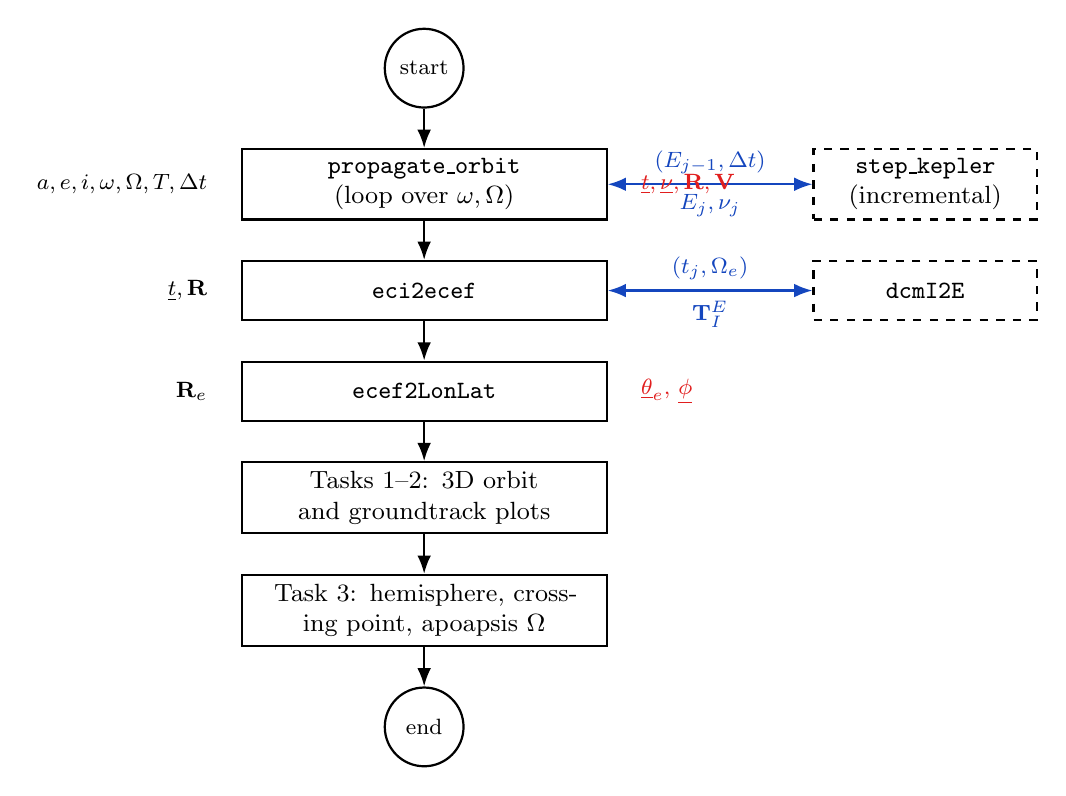
\begin{tikzpicture}[
    >=Latex, font=\small, node distance=0.5cm,
    term/.style={circle, draw, thick, minimum size=1.0cm, inner sep=1pt, font=\footnotesize},
    proc/.style={rectangle, draw, thick, minimum height=0.75cm, text width=4.4cm, align=center},
    sub/.style={rectangle, draw, thick, dashed, minimum height=0.75cm, text width=2.6cm, align=center},
    io/.style={font=\footnotesize, align=left},
]
    \node[term] (start) {start};
    \node[proc, below=of start] (prop) {\texttt{propagate\_orbit}\\(loop over $\omega,\Omega$)};
    \node[proc, below=of prop] (ecef) {\texttt{eci2ecef}};
    \node[proc, below=of ecef] (ll) {\texttt{ecef2LonLat}};
    \node[proc, below=of ll] (t12) {Tasks 1--2: 3D orbit and groundtrack plots};
    \node[proc, below=of t12] (t3) {Task 3: hemisphere, crossing point, apoapsis $\Omega$};
    \node[term, below=of t3] (end) {end};

    \node[sub, right=2.6cm of prop] (kep) {\texttt{step\_kepler}\\(incremental)};
    \node[sub, right=2.6cm of ecef] (dcm) {\texttt{dcmI2E}};

    \foreach \a/\b in {start/prop, prop/ecef, ecef/ll, ll/t12, t12/t3, t3/end}
        \draw[->, thick] (\a) -- (\b);
    \draw[<->, thick, hwblue] (prop) -- node[above, io] {$(E_{j-1},\Delta t)$} node[below, io] {$E_j,\nu_j$} (kep);
    \draw[<->, thick, hwblue] (ecef) -- node[above, io] {$(t_j,\Omega_e)$} node[below, io] {$\mathbf{T}_I^E$} (dcm);

    % inputs (left) and outputs (right of the main column)
    \node[io, left=0.3cm of prop] {$a,e,i,\omega,\Omega,T,\Delta t$};
    \node[io, left=0.3cm of ecef] {$\vect{t},\mathbf{R}$};
    \node[io, left=0.3cm of ll] {$\mathbf{R}_e$};
    \node[io, hwred, right=0.3cm of prop] {$\vect{t},\vect{\nu},\mathbf{R},\mathbf{V}$};
    \node[io, hwred, right=0.3cm of ll] {$\vect{\theta}_e,\,\vect{\phi}$};
\end{tikzpicture}
}
\caption{Program flow of \texttt{\newtxt{tasks1to3.py}}.}
\label{fig:t1-flow}
\end{figure}

\subsection*{Task 1-4: Orbits in three dimensions}

The three columns of $\mathbf{R}$ are plotted over an Earth sphere of radius $R_e = \SI{6378.1363}{\kilo\meter}$ (\texttt{earthSphere}, a Python version of \texttt{earthSphere.m} textured with a NASA equirectangular image~\cite{nasa-image}), with line width 2 and \texttt{view(49.5, 22.8)}\newtxt{, one color per value of $\Omega$, and one figure per value of $\omega$ (\cref{fig:t1-orbits})}. The Earth is drawn at $t = 0$, when $ECI$ and $ECEF$ are aligned.

\begin{figure}[H]
\centering
\begin{subfigure}{0.49\textwidth}
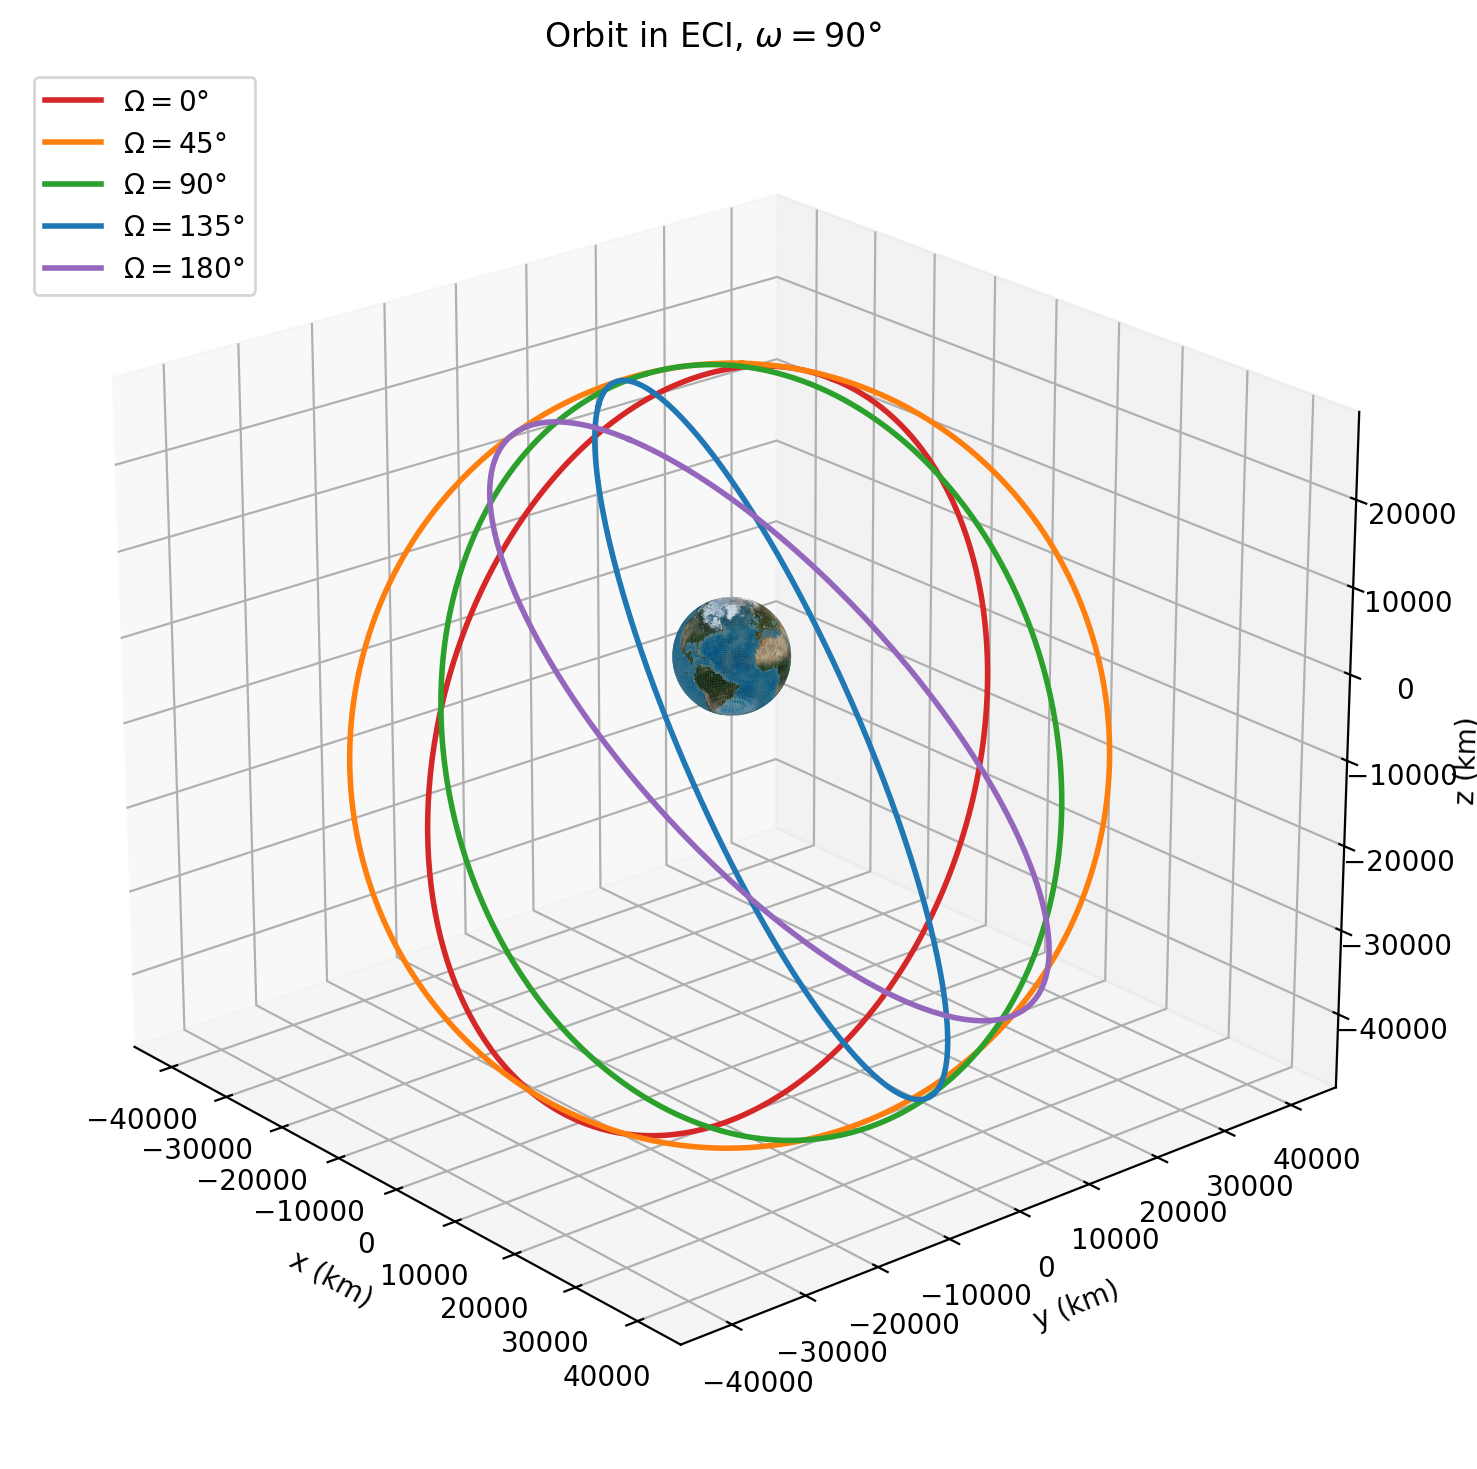
\includegraphics[width=\textwidth]{orbit3d_w90.png}
\caption{\newtxt{$\omega = 90^\circ$}}
\end{subfigure}
\hfill
\begin{subfigure}{0.49\textwidth}
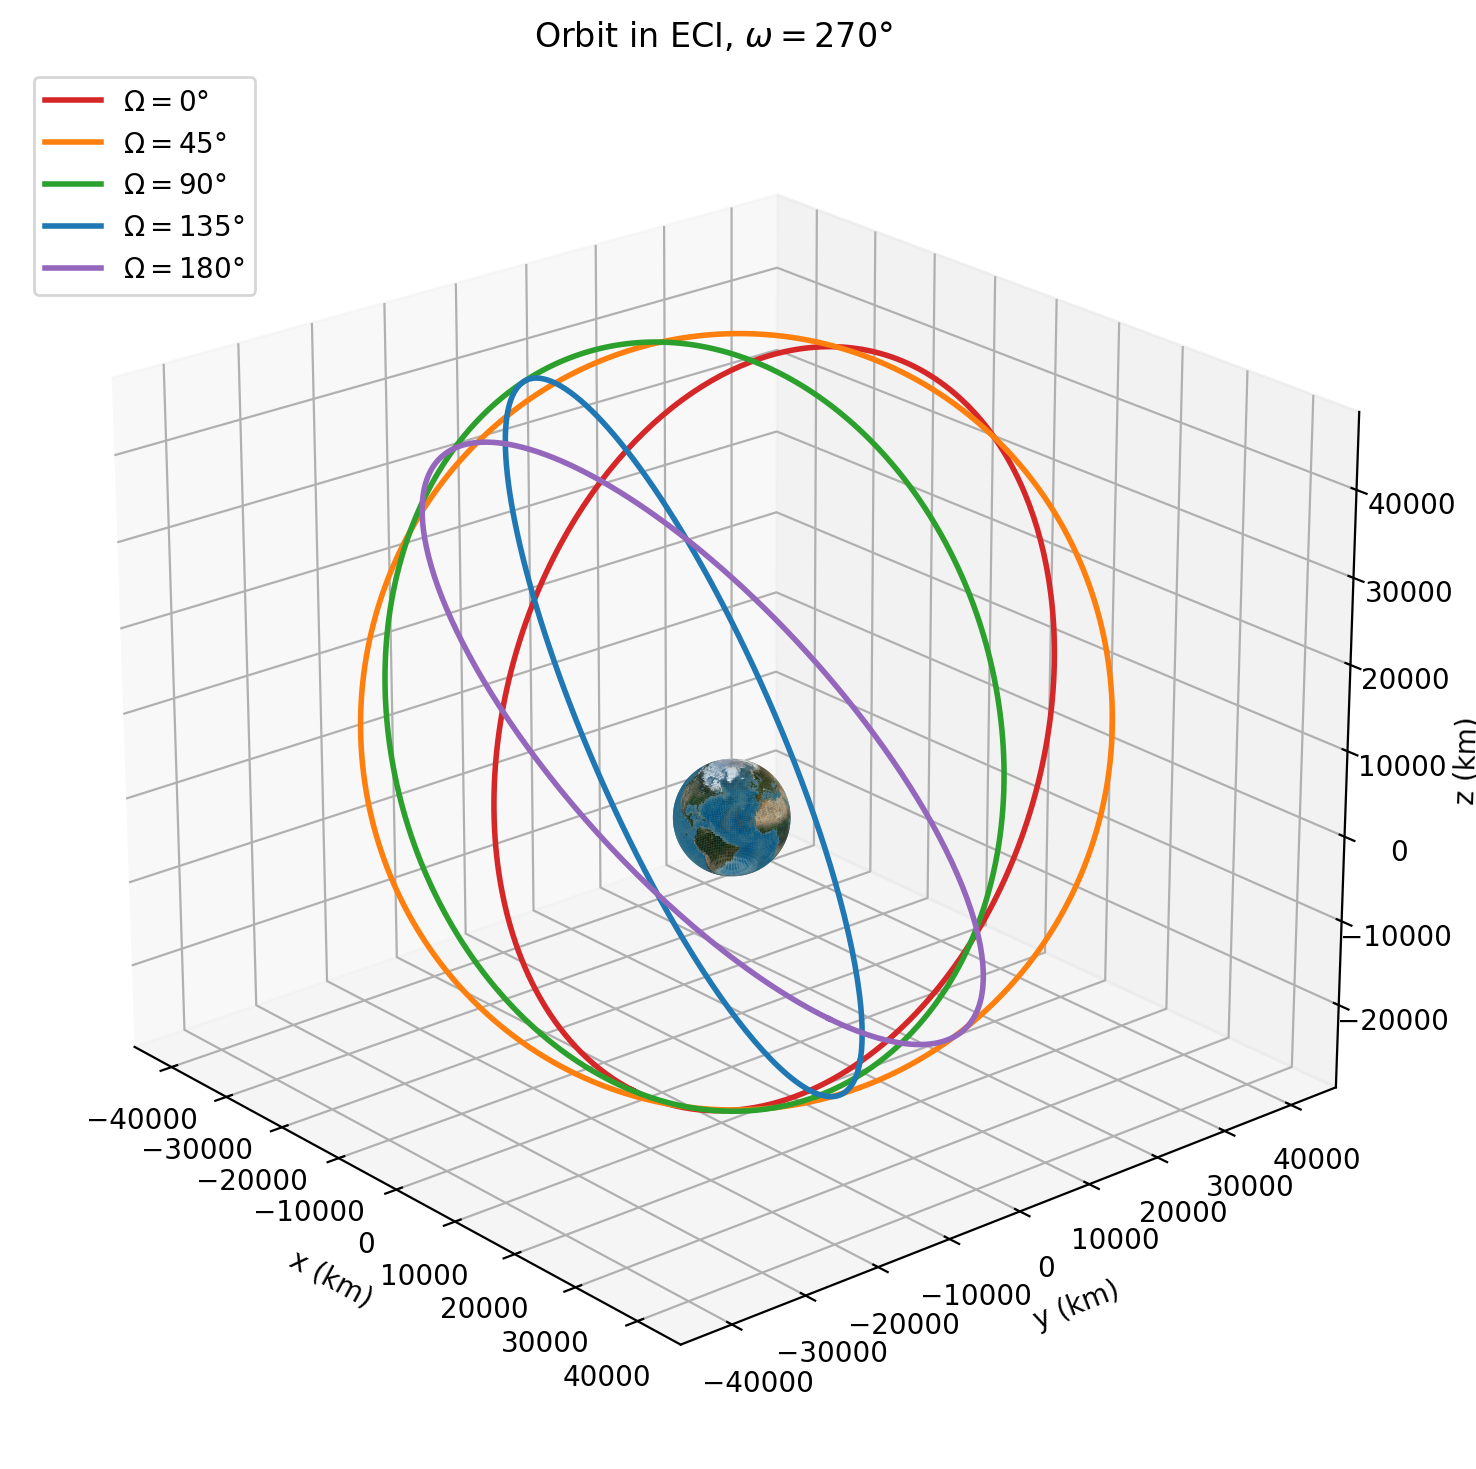
\includegraphics[width=\textwidth]{orbit3d_w270.png}
\caption{\newtxt{$\omega = 270^\circ$}}
\end{subfigure}
\caption{\newtxt{Orbit in the ECI frame over one period for $\Omega = (0,45,90,135,180)^\circ$.}}
\label{fig:t1-orbits}
\end{figure}

\subsubsection*{\newtxt{Structure of the orbit as a function of $\Omega$}}
\newtxt{Changing $\Omega$ rotates the entire orbit 'rigidly' about $\vect{I}_z$. The size, shape, and inclination of the orbit, and the latitudes of periapsis and apoapsis, do not change.}

\subsubsection*{\newtxt{Key difference between $\omega = 90^\circ$ and $\omega = 270^\circ$}}
\newtxt{For $\omega = 90^\circ$,} apoapsis ($\nu = 180^\circ$) lies \newtxt{$\omega + 180^\circ = 270^\circ$} past the ascending node, at the orbit's most \newtxt{southern} point, so the spacecraft is highest and slowest where it is farthest \newtxt{south}. \newtxt{For $\omega = 270^\circ$, apoapsis} lies $90^\circ$ past the ascending node, at the orbit's most northern point, so the spacecraft is highest and slowest where it is farthest north\newtxt{. Each orbit therefore dwells over one hemisphere.}

\FloatBarrier

\section{Task 2: Groundtrack as a Function of \texorpdfstring{$\Omega$}{Omega} and \texorpdfstring{$\omega$}{omega}}
\label{sec:task2}

The groundtrack needs the Earth-relative longitude and geocentric latitude at each $t_j$. The ECI positions in $\mathbf{R}$ are first rotated into the Earth-centered Earth-fixed (ECEF) frame $E$, which rotates about $\vect{I}_z$ at the constant rate $\Omega_e = \SI{7.2921159e-5}{\radian\per\second}$. $I$ and $E$ are aligned at $t=0$.

\begin{figure}[H]
\centering
% Redrawn from Project 2 Handwork p.5 / assignment Fig. 1 (ECI and ECEF bases, eta = Omega_e t).
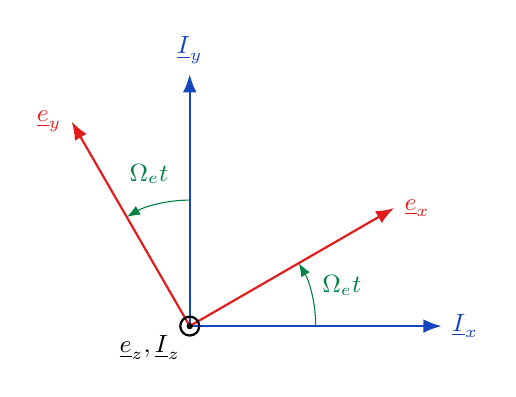
\begin{tikzpicture}[>=Latex, scale=1.0, font=\small]
    \def\ang{30}
    % ECI basis
    \draw[->, thick, hwblue] (0,0) -- (3.2,0) node[right] {$\vect{I}_x$};
    \draw[->, thick, hwblue] (0,0) -- (0,3.2) node[above] {$\vect{I}_y$};
    % ECEF basis
    \draw[->, thick, hwred] (0,0) -- (\ang:3.0) node[right] {$\vect{e}_x$};
    \draw[->, thick, hwred] (0,0) -- (90+\ang:3.0) node[left] {$\vect{e}_y$};
    % common z axis (out of page)
    \draw[thick] (0,0) circle (0.12);
    \fill (0,0) circle (0.04);
    \node[below left] at (0,0) {$\vect{e}_z,\vect{I}_z$};
    % rotation angles
    \draw[->, hwgreen] (1.6,0) arc (0:\ang:1.6);
    \node[hwgreen] at (15:2.0) {$\Omega_e t$};
    \draw[->, hwgreen] (0,1.6) arc (90:90+\ang:1.6);
    \node[hwgreen] at (105:2.0) {$\Omega_e t$};
\end{tikzpicture}

\caption{ECI basis $I = \{\vect{I}_x,\vect{I}_y,\vect{I}_z\}$ and ECEF basis $E = \{\vect{e}_x,\vect{e}_y,\vect{e}_z\}$, rotated by $\eta \equiv \Omega_e t$ about $\vect{I}_z = \vect{e}_z$.}
\label{fig:t2-frames}
\end{figure}

\subsection*{Task 2-1: Transformation from ECI to ECEF}

\paragraph{(a)} From \cref{fig:t2-frames}, with $\eta = \Omega_e t$, the ECEF basis vectors in ECI components are
\begin{equation}
\vect{e}_x = \cos\eta\,\vect{I}_x + \sin\eta\,\vect{I}_y,
\qquad
\vect{e}_y = -\sin\eta\,\vect{I}_x + \cos\eta\,\vect{I}_y,
\qquad
\vect{e}_z = \vect{I}_z.
\end{equation}
Each row of $\mathbf{T}_I^E$ holds one ECEF basis vector, so that $x_e = \vect{r}\cdot\vect{e}_x$, $y_e = \vect{r}\cdot\vect{e}_y$, $z_e = \vect{r}\cdot\vect{e}_z$:
\begin{equation}
\boxed{\mathbf{T}_I^E(t) =
\begin{bmatrix} c_{xx} & c_{xy} & c_{xz} \\ c_{yx} & c_{yy} & c_{yz} \\ c_{zx} & c_{zy} & c_{zz} \end{bmatrix}
=
\begin{bmatrix} \cos(\Omega_e t) & \sin(\Omega_e t) & 0 \\ -\sin(\Omega_e t) & \cos(\Omega_e t) & 0 \\ 0 & 0 & 1 \end{bmatrix}}.
\label{eq:t2-dcm}
\end{equation}

\paragraph{(b)} \texttt{dcmI2E(t, O\_e)} returns \cref{eq:t2-dcm}, with $t$ in \si{\second} and $\Omega_e$ in \si{\radian\per\second}.

\subsection*{Task 2-2: Position in ECEF coordinates}

\texttt{eci2ecef(t\_arr, r\_arr, O\_e)} builds $\mathbf{T}_I^E(t_j)$ at each time and applies it to the matching row of $\mathbf{R}$:
\begin{equation}
\vect{r}_e(t_j) = \mathbf{T}_I^E(t_j)\,\vect{r}(t_j),
\qquad
\mathbf{R}_e = \begin{bmatrix} \vect{r}_e^T(t_0) \\ \vdots \\ \vect{r}_e^T(t_n) \end{bmatrix} \in \mathbb{R}^{(n+1)\times 3}.
\end{equation}

\subsection*{Task 2-3: Earth-relative longitude and latitude}

With $\vect{r}_e = [x_e,\,y_e,\,z_e]$ in each row of $\mathbf{R}_e$, \texttt{ecef2LonLat(R\_ecef)} evaluates, with the four-quadrant inverse tangent,
\begin{equation}
\theta_e = \tan^{-1}(y_e,\,x_e),
\qquad
\phi = \tan^{-1}\!\left(z_e,\,\sqrt{x_e^2+y_e^2}\right).
\label{eq:t2-lonlat}
\end{equation}

\subsection*{Task 2-4: Groundtrack}

The longitudes and latitudes are converted to degrees and plotted with \texttt{mercatorDisplay} (Python version of the given code)\newtxt{, with one marker per value of $\Omega$, and one figure per value of $\omega$}. \newtxt{The} track is shown over the NASA image~\cite{nasa-image} (\newtxt{\cref{fig:t2-gt90,fig:t2-gt270}}).

\begin{figure}[H]
\centering
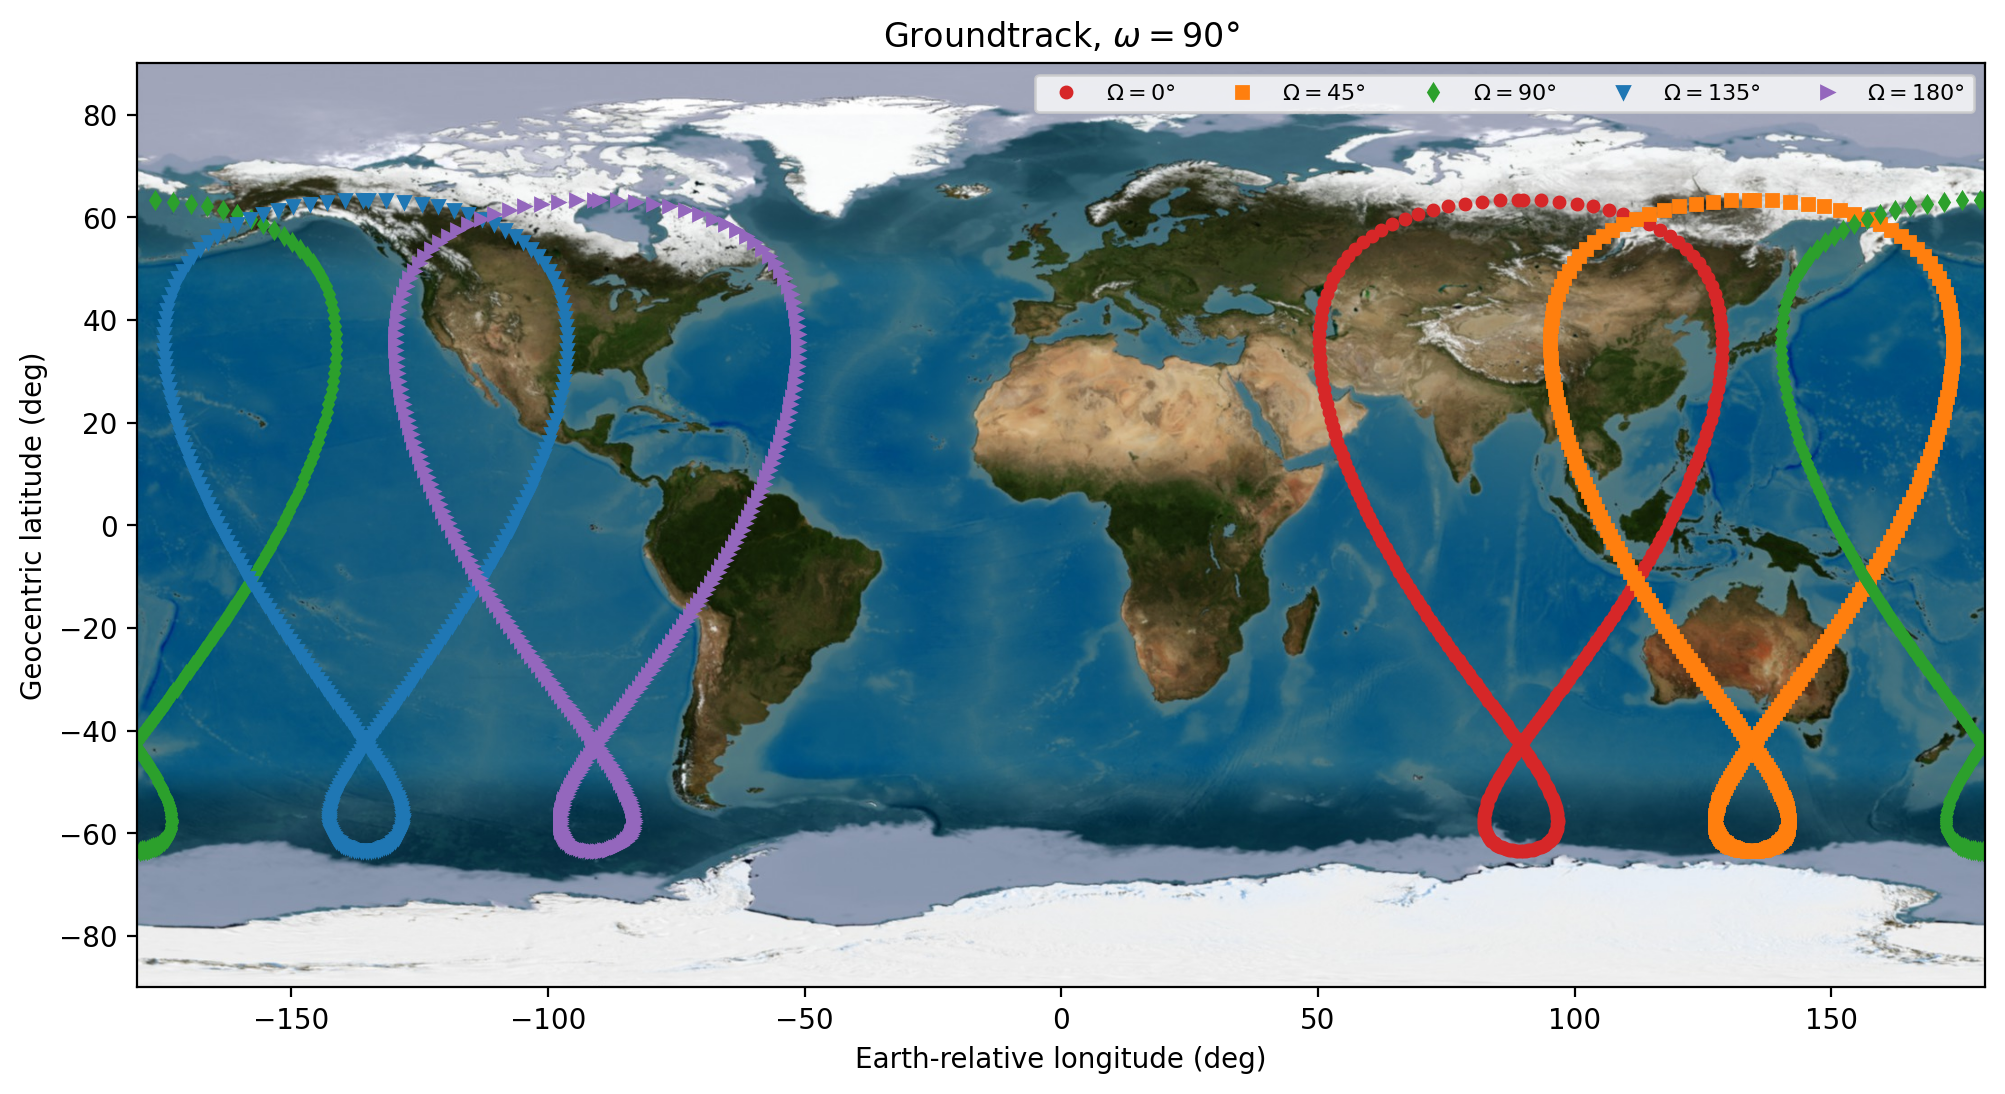
\includegraphics[width=\textwidth]{groundtrack_w90.png}
\caption{\newtxt{Groundtrack, $\omega=90^\circ$, for $\Omega=(0,45,90,135,180)^\circ$} (one marker every \SI{5}{\minute}).}
\label{fig:t2-gt90}
\end{figure}

\begin{figure}[H]
\centering
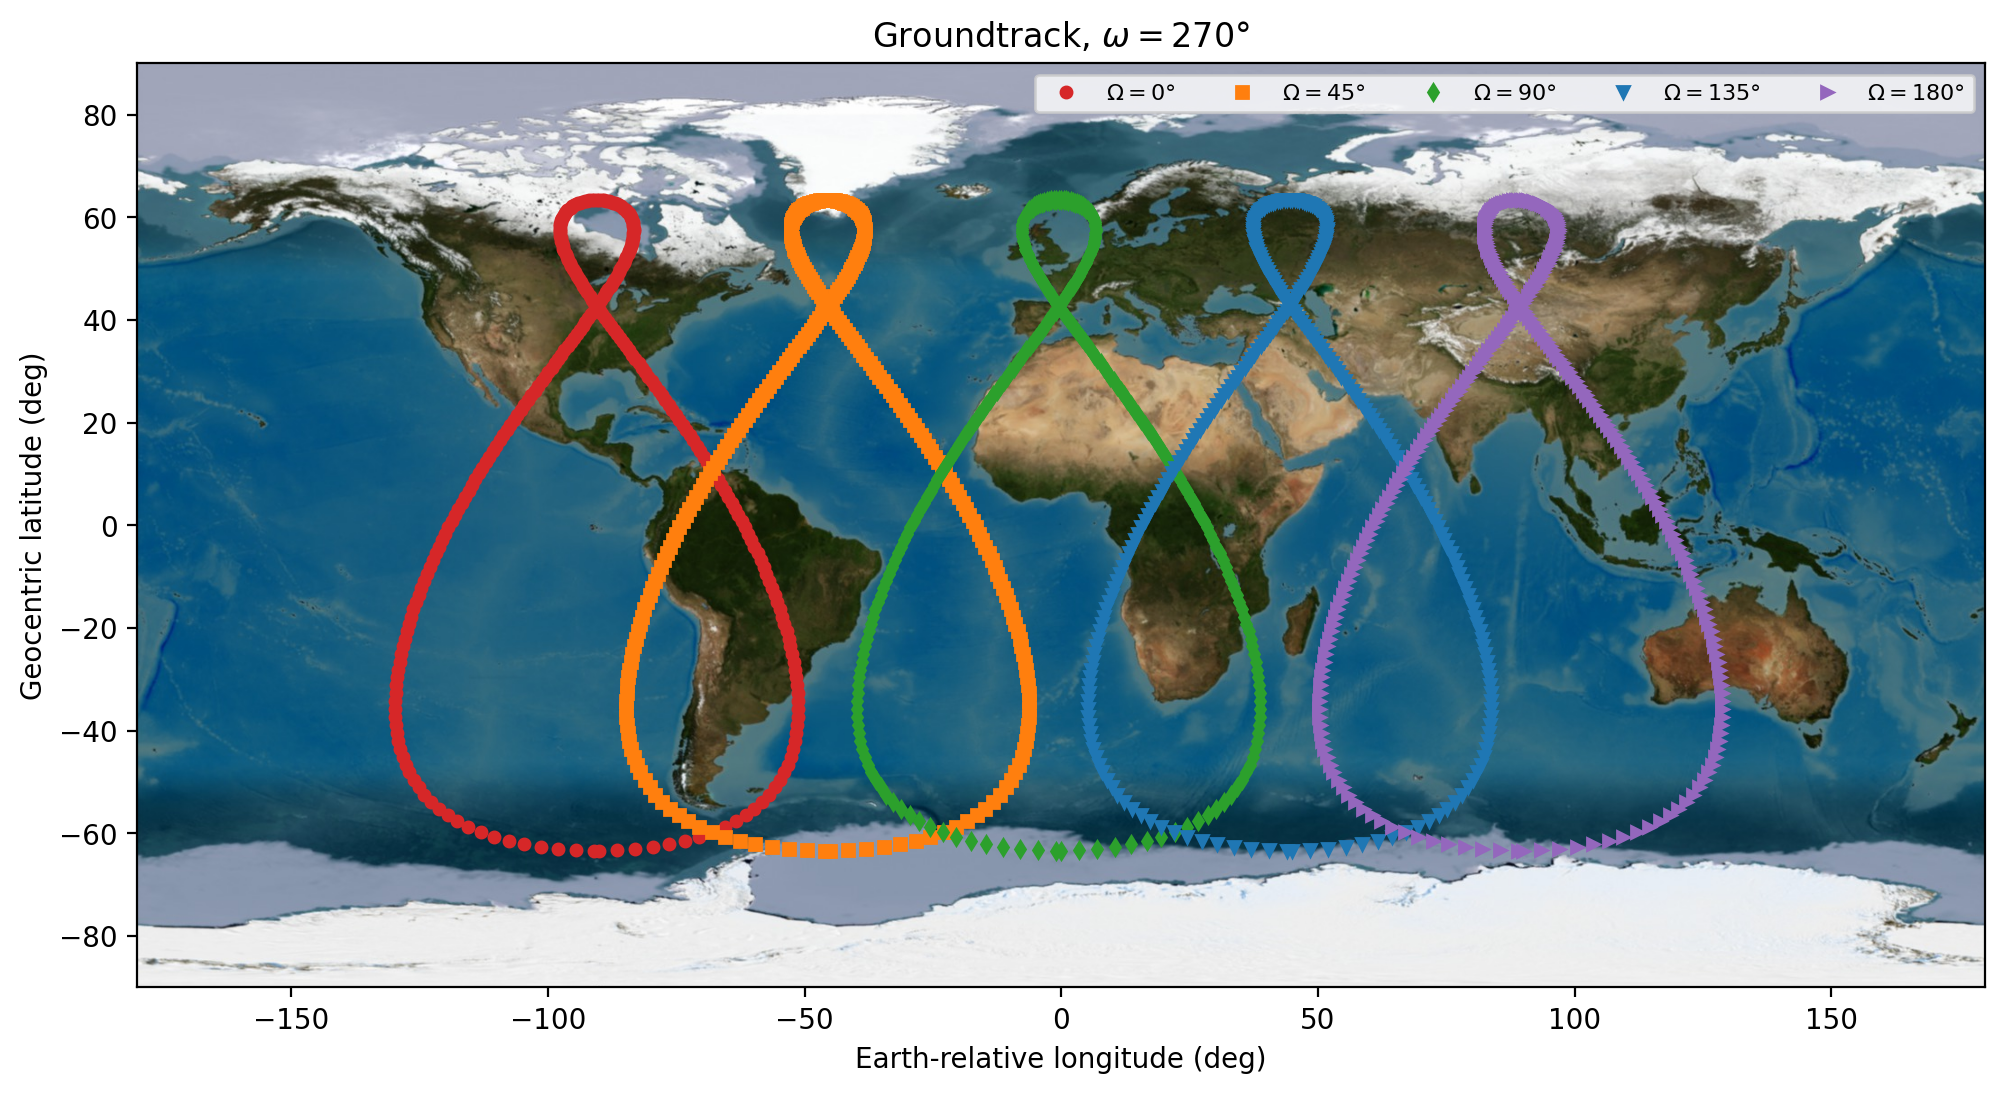
\includegraphics[width=\textwidth]{groundtrack_w270.png}
\caption{\newtxt{Groundtrack, $\omega=270^\circ$, for $\Omega=(0,45,90,135,180)^\circ$} (one marker every \SI{5}{\minute}).}
\label{fig:t2-gt270}
\end{figure}

\subsubsection*{\newtxt{Interesting feature of the groundtracks}}
\usertxt{The orbital period is $T = 24$ hours, approximately one sidereal day ($23.93$ hours). The spacecraft completes one full orbit for every rotation of the Earth, so its ground track roughly repeats in a loop, passing over the same regions at the same times. Each track looks like a figure-eight that crosses itself once, at the crossing point explained in \cref{sec:task3}. Changing $\Omega$ only shifts the track east by $\Delta\Omega$, with its shape remaining the same.}

\usertxt{Near apoapsis the spacecraft is slow and far away, tracing the small lobe of the figure-eight, and making the \SI{5}{\minute} orbit markers bunch up. Near periapsis it crosses the opposite hemisphere quickly, tracing the large lobe, and making the orbit markers appear far apart.}

\subsubsection*{\newtxt{Key difference between $\omega = 90^\circ$ and $\omega = 270^\circ$}}
\usertxt{For $\omega = 90$ deg, periapsis will always lie in the Northern hemisphere, so the apoapsis section of the figure-eight will lie in the Southern hemisphere. Since changing $\Omega$ only shifts the track east, latitudes are constant: The crossing point happens at about 43 deg, with peak apoapsis at 63.4 deg S and periapsis at 63.4 deg N. The same values are true, but in reverse for $\omega = 270$ deg (which is 180 deg apart, and thus places apoapsis in the exact opposite hemisphere).}

\FloatBarrier

\section{Task 3: Hemisphere Dwell, Crossing Point, and Apoapsis Placement}
\label{sec:task3}

\begin{newpar}
\usertxt{Because $\Omega$ only shifts the groundtrack in longitude (\cref{sec:task2}), the results from this first part will only depend on $i$, $e$, $T$, and $\omega$. To simplify, we define $\zeta = \omega + \nu$, which is the angle from the ascending node to the spacecraft. We can rotate $\vect{r}_P$ to get the ECI position:}
\begin{equation}
\begin{split}
\vect{r} &= \mathbf{R}_3(\Omega)\,\mathbf{R}_1(i)\,\mathbf{R}_3(\omega)\,\vect{r}_P \\
&= r\begin{bmatrix} \cos\Omega\cos\zeta - \sin\Omega\cos i\sin\zeta \\ \sin\Omega\cos\zeta + \cos\Omega\cos i\sin\zeta \\ \sin i\sin\zeta \end{bmatrix}.
\end{split}
\label{eq:t3-r}
\end{equation}
\usertxt{And because ECI and ECEF both share the Z component, the geocentric latitude of any point in the orbit is defined as:}
\begin{equation}
\sin\phi = \frac{z_e}{r} = \frac{z}{r} = \sin i \,\sin\zeta.
\label{eq:t3-lat}
\end{equation}

\begin{figure}[H]
\centering
% Geocentric latitude phi at a point on the orbit (schematic, not to scale).
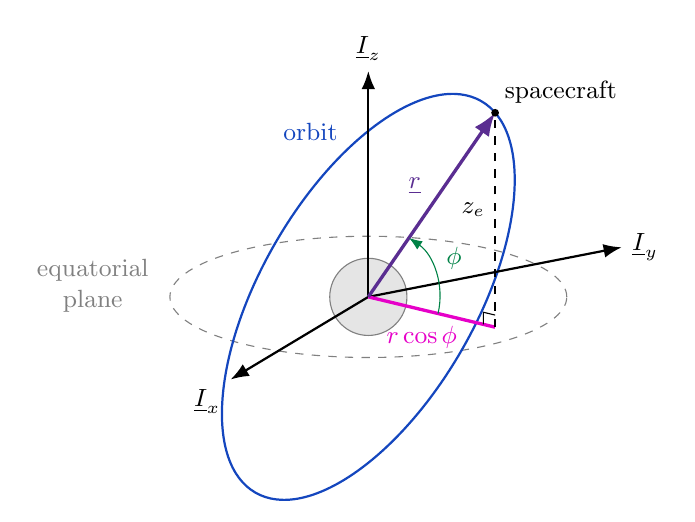
\begin{tikzpicture}[>=Latex, scale=0.7, font=\small]
    \coordinate (O) at (0,0);
    \coordinate (F) at (2.3,-0.55); % foot of the perpendicular in the equatorial plane
    \coordinate (S) at (2.3,3.34);  % spacecraft

    % Earth and equatorial plane
    \fill[gray!20] (O) circle (0.7);
    \draw[gray] (O) circle (0.7);
    \draw[dashed, gray] (O) ellipse (3.6 and 1.1);
    \node[gray, align=center] at (-5.0,0.2) {equatorial\\plane};

    % orbit
    \draw[thick, hwblue, rotate=60] (O) ellipse (4.1 and 1.95);
    \node[hwblue] at (-1.05,3.0) {orbit};

    % ECI axes
    \draw[->, thick] (O) -- (0,4.1) node[above] {$\vect{I}_z$};
    \draw[->, thick] (O) -- (-2.5,-1.5) node[below left] {$\vect{I}_x$};
    \draw[->, thick] (O) -- (4.6,0.9) node[right] {$\vect{I}_y$};

    % the latitude triangle
    \draw[very thick, hwmagenta] (O) -- (F);
    \node[hwmagenta] at (0.97,-0.73) {$r\cos\phi$};
    \draw[thick, dashed] (F) -- (S) node[pos=0.55, left] {$z_e$};
    \draw[very thick, hwpurple, ->] (O) -- (S) node[midway, above left] {$\vect{r}$};
    \draw (2.086,-0.499) -- (2.086,-0.279) -- (2.3,-0.33);

    % latitude angle
    \draw[->, hwgreen] (-13.45:1.3) arc (-13.45:55.45:1.3);
    \node[hwgreen] at (24:1.7) {$\phi$};

    % spacecraft
    \fill (S) circle (2pt);
    \node[above right] at (S) {spacecraft};
\end{tikzpicture}

\caption{\newtxt{Geocentric latitude $\phi$ at a point on the orbit, from \cref{eq:t2-lonlat}. $z_e = \vect{r}\cdot\vect{I}_z$ is the height above the equatorial plane, and $r\cos\phi = \sqrt{x_e^2+y_e^2}$ is the projection of $\vect{r}$ onto that plane (not to scale).}}
\label{fig:t3-latitude}
\end{figure}

\usertxt{We can expand $\sin\zeta$ with the angle-sum identity for each value of $\omega$ provided to get an expression only in terms of the true anomaly:}

\begin{table}[H]
\centering
\caption{\newtxt{Expansion of $\sin\zeta$ for each value of $\omega$.}}
\label{tab:t3-sinzeta}
\color{newtext}
\begin{tabular}{@{}ccc@{}}
\toprule
$\omega$ & $\sin\zeta = \sin\omega\cos\nu + \cos\omega\sin\nu$ & $\sin\zeta$ \\
\midrule
$90^\circ$ & $(1)\cos\nu + (0)\sin\nu$ & $\cos\nu$ \\
$270^\circ$ & $(-1)\cos\nu + (0)\sin\nu$ & $-\cos\nu$ \\
\bottomrule
\end{tabular}
\end{table}

\noindent Since $i = 63.4^\circ$, $\sin i \approx 0.894$, and $\sin$ is an odd function ($\sin(-x) = -\sin x$):
\begin{equation}
\sin\phi \approx 0.894\,\sin\zeta.
\end{equation}
\usertxt{This means we only need to know the sign of $\sin\zeta$ to know what hemisphere the spacecraft lies in. $\cos(\nu)$ ($\omega = 90$ deg) is negative between 90 deg and 270 deg, and $-\cos(\nu)$ ($\omega = 270$ deg) is negative between 270 deg and 90 deg (passing through 0 deg)}\newtxt{, so those are the ranges where the spacecraft is in the Southern hemisphere.}

The time since periapsis to reach any $\nu$ follows directly from \cref{eq:t1-E0} and Kepler's equation, with no iteration:
\begin{equation}
t(\nu) = \frac{E - e\sin E}{n}, \qquad n = \sqrt{\mu/a^3} = \frac{2\pi}{T}, \qquad E = E(\nu) \text{ from \cref{eq:t1-E0}}.
\label{eq:t3-tnu}
\end{equation}
\end{newpar}

\subsection*{(a)}
\subsection*{(i) Majority hemisphere}

Points with \newtxt{$\phi > 0$ (or $\phi < 0$)} are marked as inside the \newtxt{Northern (or Southern) hemisphere}. Each point stands for one $\Delta t$, so the time in the \newtxt{hemisphere} is (number of points)$\cdot\Delta t$, accurate to about $\pm\Delta t$. \newtxt{The results are listed in \cref{tab:t3a}.}

\subsection*{(ii) Time from the crossing point back to the crossing point}

\begin{newpar}
The points at $\nu$ and $360^\circ - \nu$ have the same latitude (\cref{eq:t3-lat,tab:t3-sinzeta}, since $\cos\nu$ is even). The crossing point occurs at the true anomaly $\nu_c$ where these points also have the same Earth-relative longitude, with $\theta_e$ from \cref{eq:t2-lonlat} at the time $t(\nu)$ of \cref{eq:t3-tnu}:
\begin{equation}
\boxed{\theta_e(\nu_c) = \theta_e(360^\circ-\nu_c)}.
\label{eq:t3-crossing}
\end{equation}
Since $\nu_c$ cannot be found analytically, it is solved numerically as a root-finding problem,
\begin{equation}
\theta_e(\nu_c) - \theta_e(360^\circ-\nu_c) = 0.
\end{equation}
\texttt{scipy.optimize.brentq}~\cite{scipy-brentq} is used because it is a bracketing method that only needs an interval where this difference changes sign, with no derivative. The interval is the pair of neighboring five-minute points in $\vect{N}$ where the sign changes. This gives $\nu_c = 139.31^\circ$, so the two passes are at $\nu = 139.31^\circ$ and $\nu = 220.69^\circ$. These $\nu$'s bound apoapsis, so the time from the crossing point back to it in the majority hemisphere is
\begin{equation}
\boxed{t(220.69^\circ) - t(139.31^\circ) = \SI{8.31}{\hour}}.
\end{equation}
\end{newpar}

\begin{table}[H]
\centering
\caption{\newtxt{Part (a) results.}}
\label{tab:t3a}
\color{newtext}
\begin{tabular}{@{}lrr@{}}
\toprule
Quantity & $\omega=90^\circ$ & $\omega=270^\circ$ \\
\midrule
Majority hemisphere & Southern & Northern \\
Time from crossing point back to crossing point [\si{\hour}] & $8.31$ & $8.31$ \\
\bottomrule
\end{tabular}
\end{table}

\subsection*{(b) $\Omega$ placing apoapsis over Australia and South America ($\omega=90^\circ$)}

\begin{newpar}
As stated before, changing $\Omega$ only shifts the track longitudinally, so the $\Omega$ that places apoapsis ($\nu=180^\circ$, $t = T/2$) over a target longitude $\theta_t$ can be defined as a translation from $\Omega = 0$:
\begin{equation}
\boxed{\Omega = \Big(\theta_t - \theta_e\big|_{\nu=180^\circ,\ \Omega=0}\Big) - 360^\circ\left\lfloor \frac{\theta_t - \theta_e\big|_{\nu=180^\circ,\ \Omega=0}}{360^\circ} \right\rfloor}.
\label{eq:t3-omega-apo}
\end{equation}
For $\omega=90^\circ$, apoapsis is in the Southern hemisphere and $\theta_e = 89.51^\circ$ for $\Omega = 0$. Since $0 \le \Omega \le 180^\circ$ (\cref{eq:t1-given}), any value from \cref{eq:t3-omega-apo} outside that range is replaced by the closest allowed value. The rough reference longitudes in \cref{tab:t3b} give the values of $\Omega$ and the resulting apoapsis longitudes. For South America, this limit leaves apoapsis west of the continent.
\end{newpar}

\begin{table}[H]
\centering
\caption{\newtxt{Part (b) results, $\omega=90^\circ$.}}
\label{tab:t3b}
\color{newtext}
\begin{tabular}{@{}lrrr@{}}
\toprule
Target & Rough reference longitude [\si{\degree}] & $\Omega$ [\si{\degree}] & Apoapsis longitude [\si{\degree}] \\
\midrule
Australia & $135.0$ & $45.4928$ & $135.00$ \\
South America & $-60.0$ & $180.0000$ & $-90.49$ \\
\bottomrule
\end{tabular}
\end{table}

\subsection*{(c) $\Omega$ placing apoapsis over Russia and North America ($\omega=270^\circ$)}

\begin{newpar}
\Cref{eq:t3-omega-apo} applies with $\omega=270^\circ$, where apoapsis is in the Northern hemisphere, and $\theta_e = -90.49^\circ$ for $\Omega = 0$ in this hemisphere. Using the rough reference longitudes in \cref{tab:t3c} gives the values of $\Omega$.
\end{newpar}

\begin{table}[H]
\centering
\caption{\newtxt{Part (c) results, $\omega=270^\circ$.}}
\label{tab:t3c}
\color{newtext}
\begin{tabular}{@{}lrrr@{}}
\toprule
Target & Rough reference longitude [\si{\degree}] & $\Omega$ [\si{\degree}] & Apoapsis longitude [\si{\degree}] \\
\midrule
Russia & $90.0$ & $180.0000$ & $89.51$ \\
North America & $-100.0$ & $0.0000$ & $-90.49$ \\
\bottomrule
\end{tabular}
\end{table}


\clearpage
\subsection*{Full program output}
\programoutput{outputs/main.txt}

\FloatBarrier

\clearpage
\begin{thebibliography}{9}

\bibitem{course-notes}
EAS4510 Course Notes, University of Florida, Fall 2026.

\bibitem{nasa-orbits}
NASA Earth Observatory, ``Catalog of Earth Satellite Orbits.''
\url{https://science.nasa.gov/earth/earth-observatory/catalog-of-earth-satellite-orbits/}

\bibitem{nasa-image}
NASA Scientific Visualization Studio, ``Equirectangular Projected Earth for `LARGEST'.''
\url{https://svs.gsfc.nasa.gov/3615/}

\bibitem{scipy-brentq}
\newtxt{SciPy Documentation, ``scipy.optimize.brentq.''}
\url{https://docs.scipy.org/doc/scipy/reference/generated/scipy.optimize.brentq.html}

\end{thebibliography}


\dividerpage{Appendices}{Python Source Code}{All code and sources found in: \repolink}
\appendix
\section{Python Source Code}
\label{app:code}

\subsection{Main script --- \texttt{main.py}}
\lstinputlisting[caption={Tasks 1 to 3: propagation, groundtracks, plots, and hemisphere/crossing-point/apoapsis analysis.}]{../main.py}

\clearpage
\subsection{Orbital elements --- \texttt{elements.py}}
\lstinputlisting[caption={Orbital elements to ECI position and velocity: \texttt{elements\_to\_rv}.}]{../elements.py}

\subsection{Incremental Kepler solver --- \texttt{kepler.py}}
\lstinputlisting[caption={Task 1-1: \texttt{step\_kepler}, Newton's method on Kepler's equation.}]{../kepler.py}

\subsection{Orbit propagation --- \texttt{propagate\_orbit.py}}
\lstinputlisting[caption={Task 1-2: \texttt{propagate\_orbit}.}]{../propagate_orbit.py}

\subsection{ECI to ECEF matrix --- \texttt{dcmI2E.py}}
\lstinputlisting[caption={Task 2: \texttt{dcmI2E}.}]{../dcmI2E.py}

\subsection{ECEF position --- \texttt{eci2ecef.py}}
\lstinputlisting[caption={Task 2: \texttt{eci2ecef}.}]{../eci2ecef.py}

\subsection{Longitude and latitude --- \texttt{ecef2LonLat.py}}
\lstinputlisting[caption={Task 2: \texttt{ecef2LonLat}.}]{../ecef2LonLat.py}

\clearpage
\subsection{Plotting --- \texttt{plotting.py}}
\lstinputlisting[caption={Tasks 1 and 2: \texttt{earthSphere}, \texttt{plotOrbits3D}, and \texttt{mercatorDisplay}.}]{../plotting.py}


\end{document}
